\documentclass[12pt]{extarticle}
\usepackage[utf8]{inputenc}
\usepackage[margin=1in]{geometry}
\usepackage[title]{appendix}
\usepackage{graphicx, listings, titlesec, cite, authblk, mdframed, floatrow}

\titleformat{\section}
  {\normalfont\fontsize{12}{15}\bfseries}{\thesection}{1em}{}

\title{Deep in the Web: using deep learning methods to predict Problematic Internet Use in today's youth}
\author[1]{Evan Matthews}
\author[1]{Vikram Ramavarapu}
\author[1]{Krishnaveni Unnikrishnan}
\affil[1]{CS 412 Group G6}
\date{December 11, 2024}

% commands
\newcommand{\todo}{\textcolor{red}{TODO:}~}
\newfloatcommand{capbtabbox}{table}[][\FBwidth]

\begin{document}

\maketitle

\begin{abstract}
    The Internet's pervasive role in modern life has raised concerns about Problematic Internet Use (PIU), particularly among children and teens. 
    Our research aims to predict early signs of PIU using machine learning techniques applied to data from the Child Mind Institute's Healthy Brain Network. 
    This study employs a comprehensive methodology combining both cross-sectional and time-series data for future analysis. 
    Initial results from multiple models, including Random Forest, XGBoost, SVM, and Feed Forward Neural Networks, demonstrate promising accuracy rates, with XGBoost achieving the highest mean accuracy of 0.682. 
    Our project experimentation is structured in three phases: data preprocessing, initial model evaluation, and fine-feature reevaluation. 
    The methodology incorporates innovative approaches such as sequential modeling for time-series data and ensemble techniques combining cross-sectional and sequential models. 
    Preliminary findings suggest that machine learning can effectively predict PIU severity using quantitative measures compared to traditional assessments. 
    This research contributes to the growing field of digital health by providing a data-driven approach to identifying at-risk youth for PIU.
\end{abstract}

\pagebreak

\section{Introduction}

  The Internet has become an integral part of our daily lives, with people of all ages spending a significant amount of time online. 
  This trend has given rise to concerns about the potential impacts of excessive internet use, particularly on children and teens.
  Problematic Internet Use (PIU) is a condition characterized by excessive or poorly controlled preoccupations, urges, or behaviors regarding computer use and internet access that lead to impairment or distress \cite{Pettorruso2020-qt}. 
  PIU has been associated with a range of mental health issues, including depression, anxiety, and impulsivity \cite{Cash2012-rb}.
  As such, identifying early signs of PIU in children and teens is crucial for prevention and intervention.
  Despite having multiple studies showing the negative effects of excessive internet use, exact details about PIU warning signs and the most at-risk individuals are still unknown.
  These studies can be useful, but they also introduce biases and often fail to show the true factors which correlate a participant's estimated internet impact \cite{Restrepo2020-pb,Aboujaoude2010-mc}.
  In this project, we aim to predict early signs of PIU in children and teens using machine learning techniques, leveraging data from the Child Mind Institute's Healthy Brain Network.
  The project plan consists of three phases: data preprocessing, initial model evaluation, and fine-feature reevaluation.
  We will submit our work to the Child Mind Institute's (CMI) Kaggle competition on PIU prediction, and we also aim to publish our results as a paper should they outperform competition expectations.

\section{Motivation}

  With the rise of machine learning and pattern prediction models, the ability to analyze and predict upon more complex data and parameters becomes much more approachable.
  Likewise, child development is a multi-facted situation in which parenting and environmental factors can lead to an incredibly high number of outcomes.
  This field has had great strides in classical research, but a more modern approach could lead to significant development in the success of future generations.
  Additionally, predictions against an extensive number of possible outcomes like this represents a current roadblock in machine learning- that is, how modern predictive models can adapt to an ever-increasing set of parameters and decreasing set of training data.
  Finally, child psychology is interested in recognizing patterns in early behavior in order to reduce the impact of harmful effects from a child's environment.

  Despite having multiple studies showing the negative effects of excessive internet use, exact details about PIU warning signs and the most at-risk individuals are still unknown.
  These studies can be useful, but their results focus primarily on written or binary feedback from students or parents. 
  These studies can be useful, but they also introduce biases and often fail to show the true factors which correlate a participant's estimated internet impact \cite{Restrepo2020-pb,Aboujaoude2010-mc}.

  Another major drawback of assessing PIU is in its subjective nature. 
  Problematic internet use is characterized by many different variables that are hard to measure. 
  As such, using quantitative measures such as the Severity Impairment Index (SII) allow for the application of data mining methods to aid in the classification of PIU severity. 
  Moreover, other measurable attributes such as sleep quality and duration, physical activity level, and duration of internet usage can all be used to understand correlations with PIU.
  This project intends to rectify these issues by using a machine-learning approach to predict early signs of PIU using a wider range of variables on children and teens.

\section{Related Work}

  Research on Problematic Internet Use (PIU) has gained significant attention due to its increasing prevalence and association with various psychological and behavioral issues. 
  Early investigations into PIU highlighted its similarities with substance use disorders, impulse control disorders, and obsessive-compulsive disorder.
  Studies have revealed concerning prevalence rates between 1.5\% and 8.2\% in the United States and Europe, emphasizing the growing social impact of this condition \cite{Cash2012-rb}. 
  The relationship between PIU and psychiatric disorders has been extensively documented, with research showing significant associations with depressive disorders and attention-deficit/hyperactivity disorder (ADHD). 
  A notable study found that individuals with PIU were more than twice as likely to have depressive disorders $(aOR = 2.43)$, and showed increased likelihood of having ADHD combined presentation $(aOR = 1.91)$ and Autism Spectrum Disorder $(aOR = 2.24)$ \cite{Restrepo2020-pb}.

  Recent investigations have focused on understanding the personality profiles and emotional factors contributing to PIU. Research has identified specific personality traits associated with PIU, including lower scores in novelty seeking, harm avoidance, and reward dependence. 
  Additionally, emotional dysregulation has emerged as a significant factor, with studies suggesting that PIU may serve as a behavioral mechanism for escaping negative affects.
  Treatment approaches for PIU have primarily centered on addressing comorbid conditions, with cognitive behavioral therapy and selective serotonin reuptake inhibitors showing promise as potential interventions.
  However, researchers emphasize that detailed treatment guidelines require further investigation, particularly given interactions between PIU and various psychological disorders.

  Currently, the field continues to evolve, and debates haved continued regarding diagnostic criteria and classification. While the Internet's positive impact on well-being is widely acknowledged, the pathological aspects of its use remain understudied, particularly regarding subtle psychological changes such as online disinhibition. 
  This highlights the need for additional research into the pathophysiology, epidemiology, natural course, and treatment of PIU to develop more effective intervention strategies.
  In terms of our current work, given that the original scope of the project was accepted, we are pressing forward with this plan with no significant changes.
  The most crucial critique provided- that the validation plan and evaluation metric were not clear- are likewise addressed in the methodology section.

\section{Methodology}

  Data for this project has two components: cross-sectional, and time-series. The cross-sectional data is per participant and contains fields described in the following table.
  Each time-series dataset is per participant and each entry of the dataset represents the status of the participant's heartrate monitor at a given point in time. 
  PCIAT is the Parent-Child Internet Addiction Test score, which is used to compute the Severity of Internet Addiction Index (SII) score. 
  The SII score is the target variable for this project. For the description of fields in the time-series dataset, see Table \ref{table:fields}.

  The project is divided into three phases: data preprocessing, initial model evaluation, and fine-feature reevaluation.
  The data preprocessing phase entails dropping survey-based fields used to compute PCIAT, which is then used to compute the SII, as our model's intention is to compute SII directly from the other metrics.
  Missing values in the data are filled using iterative imputation, and the missing SII values are filled in using K-Nearest Neighbors $(k=5)$.

  Multiple models will be evaluated on the cross-sectional data: Random Forest, XGBoost, SVM, and a feed forward neural network. After this, a sequential model, evaluated amongst transformers or auto-encoders, will be trained on the time-series data. 
  The sequential model will allow us to compute an embedding of the time-series data, which will be used as an additional feature in the cross-sectional model.
  The final model will be an ensemble of the cross-sectional and sequential models, with the sequential model's embedding as an additional feature in the cross-sectional model. 
  The classifier model will be retrained on the concatenated dataset, to predict the SII.
  Finally, validation of the trained models is performed using 10-fold cross-validation, with the best model selected based on performance metrics.

  After comparing classifiers and selecting the best model, we land on the following methodology: first, XGBoost is trained on the cross-sectional data, where missing values are filled using label propagation. A transformer encoder is trained on the time-series data using reconstruction loss, and the encoder is used to compute an embedding of the time-series data. The embedding is concatenated with the cross-sectional data, and the XGBoost model is retrained on the concatenated dataset. In the testing phase, for a datapoint that has a time-series component, the transformer encoder is used to compute the embedding, which is then concatenated with the cross-sectional data and fed into the XGBoost model to predict the SII. If time-series data is not available, the XGBoost model is used to predict the SII directly from the cross-sectional data.

  \subsection{Results} 
  \subsubsection{Cross-Sectional Data}

    Preliminary results of 10-fold cross-validation provide insight into the performance consistency of each model - Random Forest Classifier, XGBoost Classifier, Support Vector Classifier, and Feed Forward Neural Network across different subsets of the dataset. 
    This method helps ensure that the reported accuracy is not overly dependent on any particular training subset, giving a more reliable view of how each model would perform in a real-world setting. 
    These results are summarized in Table 1 and 2.

    \begin{table}[h!]
        \centering
        \resizebox{\columnwidth}{!}{%
        \begin{tabular}{|l|c|c|c|c|c|c|c|c|c|c|c|}
            \hline
            \textbf{Model} & \textbf{Fold 1} & \textbf{Fold 2} & \textbf{Fold 3} & \textbf{Fold 4} & \textbf{Fold 5} & \textbf{Fold 6} & \textbf{Fold 7} & \textbf{Fold 8} & \textbf{Fold 9} & \textbf{Fold 10} \\
            \hline
            RF & 0.684 & 0.682 & 0.682 & 0.674 & 0.687 & 0.674 & 0.684 & 0.707 & 0.649 & 0.672 \\
            \hline
            XGB& 0.689 & 0.667 & 0.669 & 0.689 & 0.682 & 0.684 & 0.674 & 0.732 & 0.636 & 0.694 \\
            \hline
            SVC & 0.649 & 0.657 & 0.646 & 0.649 & 0.649 & 0.646 & 0.649 & 0.649 & 0.654 & 0.652 \\
            \hline
            FFN & 0.710 & 0.649 & 0.669 & 0.692 & 0.689 & 0.684 & 0.687 & 0.674 & 0.649 & 0.694 \\
            \hline
        \end{tabular}%
        }
        \caption{10-Fold Cross-Validation Results for Each Model}
        \label{table:10foldcv-results}
    \end{table}

    \begin{table}[h!]
        \centering
        \begin{tabular}{|l|c|}
            \hline
            \textbf{Model} & \textbf{Mean Accuracy} \\
            \hline
            Random Forest Classifier & 0.680 \\
            \hline
            XGBoost Classifier & 0.682 \\
            \hline
            Support Vector Classifier & 0.650 \\
            \hline
            Feed Forward Neural Network & 0.680 \\
            \hline
        \end{tabular}
        \caption{Mean Accuracy for Each Model}
        \label{'table:mean_accuracy_table'}
    \end{table}

    \begin{figure}[h!]
        \centering
        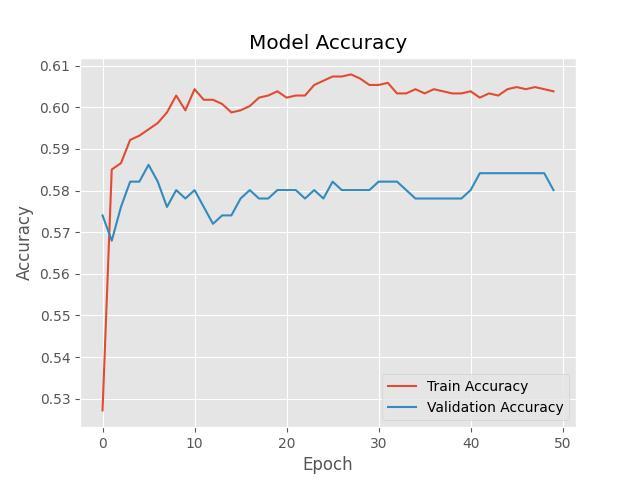
\includegraphics[scale=0.8]{"./images/model_accuracy.jpg"}
        \caption{Model accuracy of Feed-Forward Neural Network}
    \end{figure}

    Using hypothesis testing, we conclude that XGBoost model is significantly better than the other models based on a Student's t-test at significance level $\alpha=5\%$ and number of parameters to be trained.

\section{Empirical Results}

\begin{figure}[h!]
  \centering
  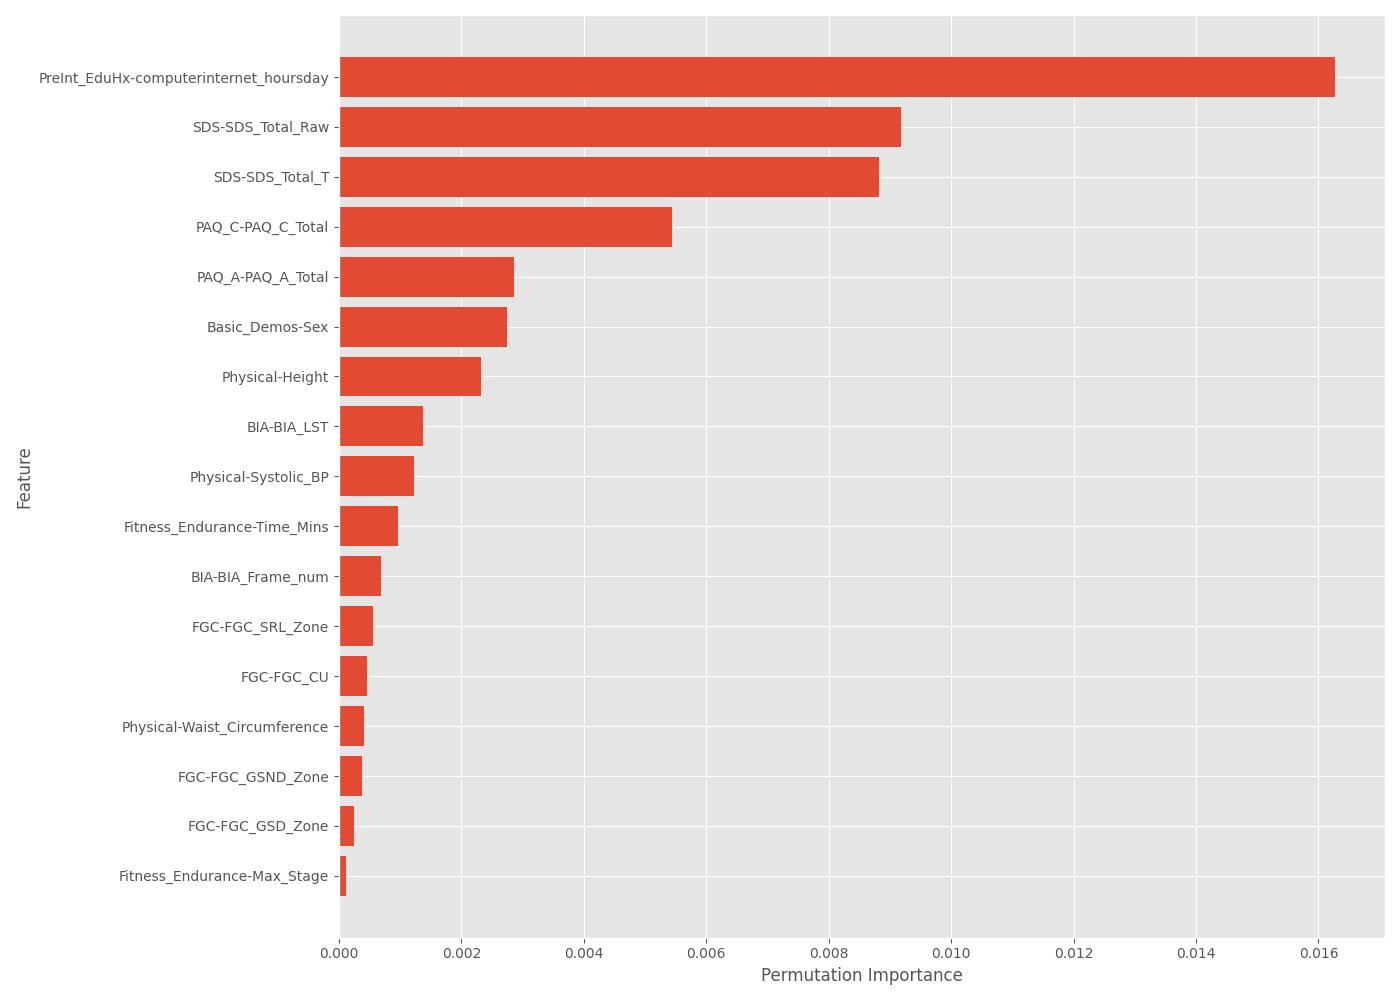
\includegraphics[scale=0.4]{"./images/feature_importance.jpg"}
  \caption{Features plotted in order of importance, ascending.}
\end{figure}


\section{Discussion and Conclusion}

\pagebreak
\nocite{*}
\bibliographystyle{plain}
\bibliography{bibliography}

\pagebreak

\begin{appendices}
    \section*{Appendix}

    % \section{Feature Importance, Feed-Forward Neural Network}
    %     \begin{figure}[h!]
    %         \centering
    %         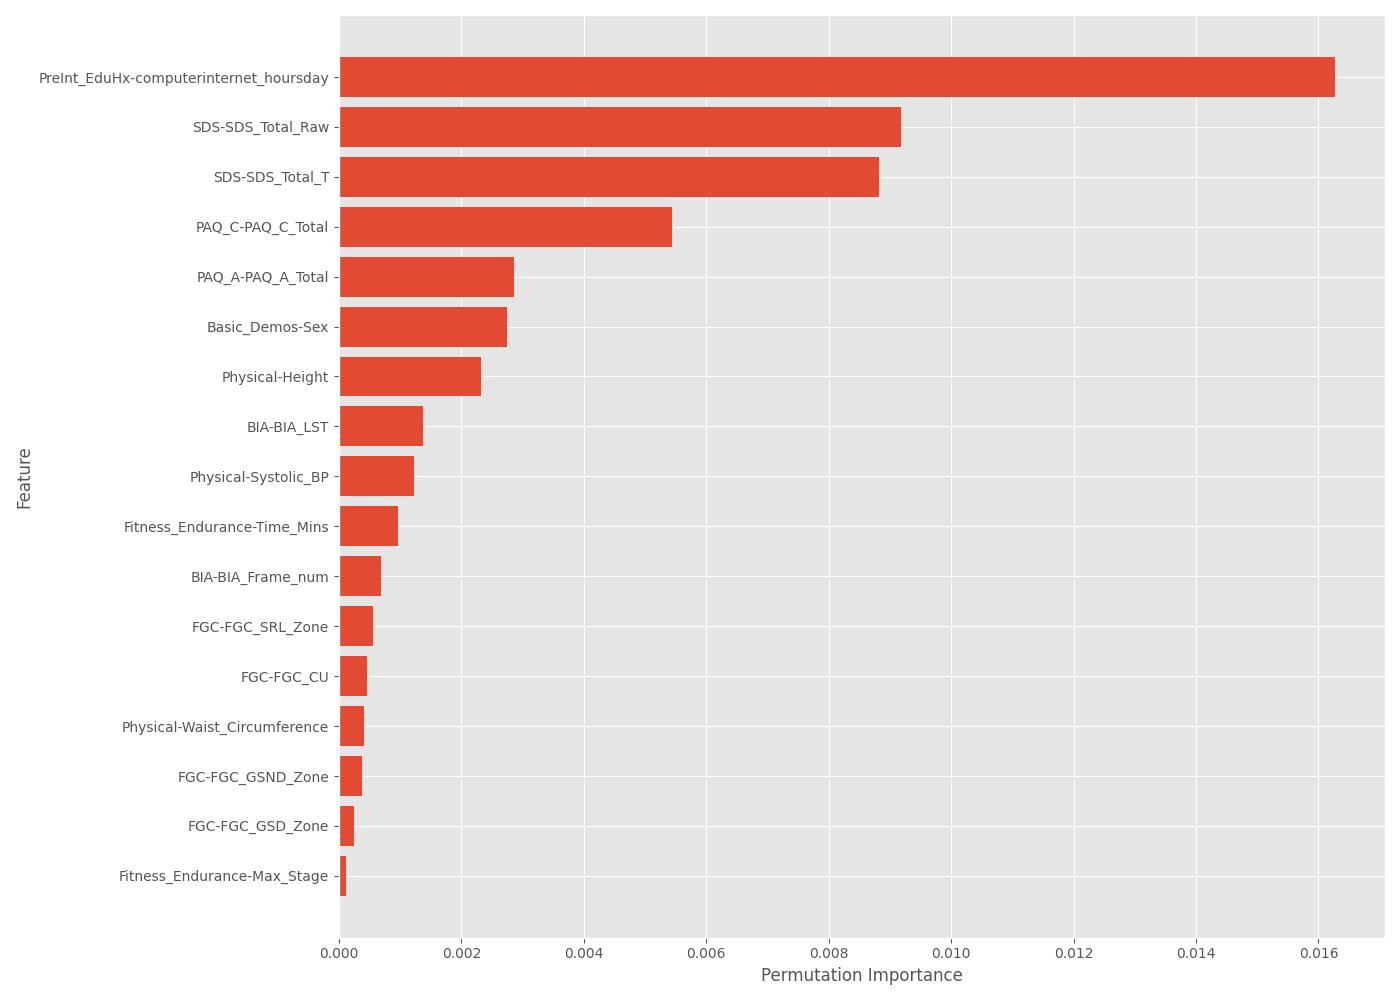
\includegraphics[scale=0.4]{"./images/feature_importance.jpg"}
    %         \caption{Features plotted in order of importance, ascending.}
    %     \end{figure}
    % \pagebreak

    \section{Description of Fields in Time-Series Dataset}
    \begin{table}[h!]
        \centering
        \begin{tabular}{|c|c|}
        \hline
        \textbf{Field} & \textbf{Description} \\
        \hline
        step & Step count \\
        X & X-axis acceleration of the heartrate monitor \\
        Y & Y-axis acceleration of the heartrate monitor \\
        Z & Z-axis acceleration of the heartrate monitor \\
        enmo & Euclidean Norm Minus One (ENMO) \\
        anglez & Angle in the Z-axis \\
        non-wear\_flag & Non-wear flag \\
        light & Light exposure \\
        battery\_voltage & Battery voltage of the monitor \\
        time\_of\_day & Time of day \\
        weekday & Day of the week \\
        quarter & Quarter of the year \\
        relative\_date\_PCIAT & Current PCIAT minus previous day PCIAT \\
        \hline
        \end{tabular}
        % \caption{Description of fields in the time-series dataset}
        \label{table:fields}
    \end{table}


    \pagebreak
    \section{Kaggle Starter Code \cite{antonina_dolgorukova_2024}}
    \begin{mdframed}
    \begin{lstlisting}[breaklines=true]
    # Starter Notebook: Multi-Target Prediction Using CatBoost

    See [this discussion](https://www.kaggle.com/competitions/child-mind-institute-problematic-internet-use/discussion/535121) for more information.
    import warnings
    from functools import partial
    from pathlib import Path

    import matplotlib.pyplot as plt
    import numpy as np
    import optuna
    import polars as pl
    import polars.selectors as cs
    from catboost import CatBoostRegressor, MultiTargetCustomMetric
    from numpy.typing import ArrayLike, NDArray
    from polars.testing import assert_frame_equal
    from sklearn.base import BaseEstimator
    from sklearn.metrics import cohen_kappa_score
    from sklearn.model_selection import StratifiedKFold

    warnings.filterwarnings("ignore", message="Failed to optimize method")

    DATA_DIR = Path("./child-mind-institute-problematic-internet-use")
    TARGET_COLS = [
        "PCIAT-PCIAT_01",
        "PCIAT-PCIAT_02",
        "PCIAT-PCIAT_03",
        "PCIAT-PCIAT_04",
        "PCIAT-PCIAT_05",
        "PCIAT-PCIAT_06",
        "PCIAT-PCIAT_07",
        "PCIAT-PCIAT_08",
        "PCIAT-PCIAT_09",
        "PCIAT-PCIAT_10",
        "PCIAT-PCIAT_11",
        "PCIAT-PCIAT_12",
        "PCIAT-PCIAT_13",
        "PCIAT-PCIAT_14",
        "PCIAT-PCIAT_15",
        "PCIAT-PCIAT_16",
        "PCIAT-PCIAT_17",
        "PCIAT-PCIAT_18",
        "PCIAT-PCIAT_19",
        "PCIAT-PCIAT_20",
        "PCIAT-PCIAT_Total",
        "sii",
    ]

    FEATURE_COLS = [
        "Basic_Demos-Enroll_Season",
        "Basic_Demos-Age",
        "Basic_Demos-Sex",
        "CGAS-Season",
        "CGAS-CGAS_Score",
        "Physical-Season",
        "Physical-BMI",
        "Physical-Height",
        "Physical-Weight",
        "Physical-Waist_Circumference",
        "Physical-Diastolic_BP",
        "Physical-HeartRate",
        "Physical-Systolic_BP",
        "Fitness_Endurance-Season",
        "Fitness_Endurance-Max_Stage",
        "Fitness_Endurance-Time_Mins",
        "Fitness_Endurance-Time_Sec",
        "FGC-Season",
        "FGC-FGC_CU",
        "FGC-FGC_CU_Zone",
        "FGC-FGC_GSND",
        "FGC-FGC_GSND_Zone",
        "FGC-FGC_GSD",
        "FGC-FGC_GSD_Zone",
        "FGC-FGC_PU",
        "FGC-FGC_PU_Zone",
        "FGC-FGC_SRL",
        "FGC-FGC_SRL_Zone",
        "FGC-FGC_SRR",
        "FGC-FGC_SRR_Zone",
        "FGC-FGC_TL",
        "FGC-FGC_TL_Zone",
        "BIA-Season",
        "BIA-BIA_Activity_Level_num",
        "BIA-BIA_BMC",
        "BIA-BIA_BMI",
        "BIA-BIA_BMR",
        "BIA-BIA_DEE",
        "BIA-BIA_ECW",
        "BIA-BIA_FFM",
        "BIA-BIA_FFMI",
        "BIA-BIA_FMI",
        "BIA-BIA_Fat",
        "BIA-BIA_Frame_num",
        "BIA-BIA_ICW",
        "BIA-BIA_LDM",
        "BIA-BIA_LST",
        "BIA-BIA_SMM",
        "BIA-BIA_TBW",
        "PAQ_A-Season",
        "PAQ_A-PAQ_A_Total",
        "PAQ_C-Season",
        "PAQ_C-PAQ_C_Total",
        "SDS-Season",
        "SDS-SDS_Total_Raw",
        "SDS-SDS_Total_T",
        "PreInt_EduHx-Season",
        "PreInt_EduHx-computerinternet_hoursday",
    ]
    # Load data
    train = pl.read_csv(DATA_DIR / "train.csv")
    test = pl.read_csv(DATA_DIR / "test.csv")
    train_test = pl.concat([train, test], how="diagonal")

    IS_TEST = test.height <= 100

    assert_frame_equal(train, train_test[: train.height].select(train.columns))
    assert_frame_equal(test, train_test[train.height :].select(test.columns))
    # Cast string columns to categorical
    train_test = train_test.with_columns(cs.string().cast(pl.Categorical).fill_null("NAN"))
    train = train_test[: train.height]
    test = train_test[train.height :]

    # ignore rows with null values in TARGET_COLS
    train_without_null = train_test.drop_nulls(subset=TARGET_COLS)
    X = train_without_null.select(FEATURE_COLS)
    X_test = test.select(FEATURE_COLS)
    y = train_without_null.select(TARGET_COLS)
    y_sii = y.get_column("sii").to_numpy()  # ground truth
    cat_features = X.select(cs.categorical()).columns
    class MultiTargetQWK(MultiTargetCustomMetric):
        def get_final_error(self, error, weight):
            return np.sum(error)  # / np.sum(weight)

        def is_max_optimal(self):
            # if True, the bigger the better
            return True

        def evaluate(self, approxes, targets, weight):
            approx = np.clip(approxes[-1], 0, 3).round().astype(int)
            target = targets[-1]

            qwk = cohen_kappa_score(target, approx, weights="quadratic")

            return qwk, 1

        def get_custom_metric_name(self):
            return "MultiTargetQWK"


    class OptimizedRounder:
        """
        A class for optimizing the rounding of continuous predictions into discrete class labels using Optuna.
        The optimization process maximizes the Quadratic Weighted Kappa score by learning thresholds that separate
        continuous predictions into class intervals.

        Args:
            n_classes (int): The number of discrete class labels.
            n_trials (int, optional): The number of trials for the Optuna optimization. Defaults to 100.

        Attributes:
            n_classes (int): The number of discrete class labels.
            labels (NDArray[np.int_]): An array of class labels from 0 to `n_classes - 1`.
            n_trials (int): The number of optimization trials.
            metric (Callable): The Quadratic Weighted Kappa score metric used for optimization.
            thresholds (List[float]): The optimized thresholds learned after calling `fit()`.

        Methods:
            fit(y_pred: NDArray[np.float_], y_true: NDArray[np.int_]) -> None:
                Fits the rounding thresholds based on continuous predictions and ground truth labels.

                Args:
                    y_pred (NDArray[np.float_]): Continuous predictions that need to be rounded.
                    y_true (NDArray[np.int_]): Ground truth class labels.

                Returns:
                    None

            predict(y_pred: NDArray[np.float_]) -> NDArray[np.int_]:
                Predicts discrete class labels by rounding continuous predictions using the fitted thresholds.
                `fit()` must be called before `predict()`.

                Args:
                    y_pred (NDArray[np.float_]): Continuous predictions to be rounded.

                Returns:
                    NDArray[np.int_]: Predicted class labels.

            _normalize(y: NDArray[np.float_]) -> NDArray[np.float_]:
                Normalizes the continuous values to the range [0, `n_classes - 1`].

                Args:
                    y (NDArray[np.float_]): Continuous values to be normalized.

                Returns:
                    NDArray[np.float_]: Normalized values.

        References:
            - This implementation uses Optuna for threshold optimization.
            - Quadratic Weighted Kappa is used as the evaluation metric.
        """

        def __init__(self, n_classes: int, n_trials: int = 100):
            self.n_classes = n_classes
            self.labels = np.arange(n_classes)
            self.n_trials = n_trials
            self.metric = partial(cohen_kappa_score, weights="quadratic")

        def fit(self, y_pred: NDArray[np.float_], y_true: NDArray[np.int_]) -> None:
            y_pred = self._normalize(y_pred)

            def objective(trial: optuna.Trial) -> float:
                thresholds = []
                for i in range(self.n_classes - 1):
                    low = max(thresholds) if i > 0 else min(self.labels)
                    high = max(self.labels)
                    th = trial.suggest_float(f"threshold_{i}", low, high)
                    thresholds.append(th)
                try:
                    y_pred_rounded = np.digitize(y_pred, thresholds)
                except ValueError:
                    return -100
                return self.metric(y_true, y_pred_rounded)

            optuna.logging.disable_default_handler()
            study = optuna.create_study(direction="maximize")
            study.optimize(
                objective,
                n_trials=self.n_trials,
            )
            self.thresholds = [study.best_params[f"threshold_{i}"] for i in range(self.n_classes - 1)]

        def predict(self, y_pred: NDArray[np.float_]) -> NDArray[np.int_]:
            assert hasattr(self, "thresholds"), "fit() must be called before predict()"
            y_pred = self._normalize(y_pred)
            return np.digitize(y_pred, self.thresholds)

        def _normalize(self, y: NDArray[np.float_]) -> NDArray[np.float_]:
            # normalize y_pred to [0, n_classes - 1]
            return (y - y.min()) / (y.max() - y.min()) * (self.n_classes - 1)
    # setting catboost parameters
    params = dict(
        loss_function="MultiRMSE",
        eval_metric=MultiTargetQWK(),
        iterations=1 if IS_TEST else 100000,
        learning_rate=0.1,
        depth=5,
        early_stopping_rounds=50,
    )

    # Cross-validation
    skf = StratifiedKFold(n_splits=5, shuffle=True, random_state=52)
    models: list[CatBoostRegressor] = []
    y_pred = np.full((X.height, len(TARGET_COLS)), fill_value=np.nan)
    for train_idx, val_idx in skf.split(X, y_sii):
        X_train: pl.DataFrame
        X_val: pl.DataFrame
        y_train: pl.DataFrame
        y_val: pl.DataFrame
        X_train, X_val = X[train_idx], X[val_idx]
        y_train, y_val = y[train_idx], y[val_idx]

        # train model
        model = CatBoostRegressor(**params)
        model.fit(
            X_train.to_pandas(),
            y_train.to_pandas(),
            eval_set=(X_val.to_pandas(), y_val.to_pandas()),
            cat_features=cat_features,
            verbose=False,
        )
        models.append(model)

        # predict
        y_pred[val_idx] = model.predict(X_val.to_pandas())

    assert np.isnan(y_pred).sum() == 0
    # Optimize thresholds
    optimizer = OptimizedRounder(n_classes=4, n_trials=300)
    y_pred_total = y_pred[:, TARGET_COLS.index("PCIAT-PCIAT_Total")]
    optimizer.fit(y_pred_total, y_sii)
    y_pred_rounded = optimizer.predict(y_pred_total)

    # Calculate QWK
    qwk = cohen_kappa_score(y_sii, y_pred_rounded, weights="quadratic")
    print(f"Cross-Validated QWK Score: {qwk}")
    feature_importance = np.mean([model.get_feature_importance() for model in models], axis=0)
    sorted_idx = np.argsort(feature_importance)
    fig = plt.figure(figsize=(12, 10))
    plt.barh(range(len(sorted_idx)), feature_importance[sorted_idx], align="center")
    plt.yticks(range(len(sorted_idx)), np.array(X_test.columns)[sorted_idx])
    plt.title("Feature Importance")
    class AvgModel:
        def __init__(self, models: list[BaseEstimator]):
            self.models = models

        def predict(self, X: ArrayLike) -> NDArray[np.int_]:
            preds: list[NDArray[np.int_]] = []
            for model in self.models:
                pred = model.predict(X)
                preds.append(pred)

            return np.mean(preds, axis=0)
    avg_model = AvgModel(models)
    test_pred = avg_model.predict(X_test.to_pandas())[:, TARGET_COLS.index("PCIAT-PCIAT_Total")]
    test_pred_rounded = optimizer.predict(test_pred)
    test.select("id").with_columns(
        pl.Series("sii", pl.Series("sii", test_pred_rounded)),
    ).write_csv("submission.csv")
    \end{lstlisting}
    \end{mdframed}


    \pagebreak
    \section{Hypothesis Testing}
    In order to compare two models A and B the null hypothesis is that the distribution of $acc(A)_i - acc(B)_i$ has zero mean and the alternative hypothesis is that the model with the higher mean performance accuarcy is significantly better than the other.\\
    T statistic is given by:
        \[
        t = \frac{\overline{acc}(A) - \overline{acc}(B)}{\sqrt{var(A - B)/k}}
        \]
        where,
        \[
        var(A - B) = \frac{1}{k}\sum_{i=1}^k [acc(A)_i - acc(B)_i - (\overline{acc}(A) - \overline{acc}(B))]^2
        \]

        \begin{table}[h!]
            \centering
            \caption{Comparison of Models using t-statistic and p-value}
            \begin{tabular}{|l|l|c|c|l|}
                \hline
                \textbf{Model 1} & \textbf{Model 2} & \textbf{t-statistic} & \textbf{p-value} & \textbf{Accept/Reject Null} \\
                \hline
                RF & XGB & -0.492 & 0.633 & Accept \\
                \hline
                RF & SVC & 6.149 & 0.0 & Reject \\
                \hline
                RF & FFN & -0.039 & 0.970 & Accept \\
                \hline
                XGB & FFN & 0.304 & 0.767 & Accept \\
                \hline
                XGB & SVC & 4.104 & 0.002 & Reject \\
                \hline
                FFN & SVC & 4.588 & 0.001 & Reject \\
                \hline
            \end{tabular}
        \end{table}
    Therefore, we can conclude that RF, XGB and FFN are significantly better than SVC. 
    However it looks like the distribution of accuracies of RF , XGB and FFN are comparable. 
    In this case we will choose the model that requires the least amount of parameters which is the XGBoost classifier.

    \pagebreak
    \section{SII Prediction Code}
    \begin{mdframed}
    \begin{lstlisting}[breaklines=true]
        import numpy as np
import torch
from torch.utils.data import Dataset, DataLoader
import pandas as pd
from sklearn.experimental import enable_iterative_imputer 
from sklearn.impute import IterativeImputer
from sklearn.semi_supervised import LabelPropagation
from sklearn.preprocessing import StandardScaler
import torch.nn as nn
import torch.optim as optim
import os
os.environ['PYTORCH_CUDA_ALLOC_CONF'] = 'max_split_size_mb:128'

def preprocess_time_series(parquet_dir, output_dir, batch_size=100):
    os.makedirs(output_dir, exist_ok=True)

    # Traverse subdirectories and collect parquet files
    patient_dirs = [d for d in os.listdir(parquet_dir) if os.path.isdir(os.path.join(parquet_dir, d))]

    for i in range(0, len(patient_dirs), batch_size):
        batch_dirs = patient_dirs[i:i + batch_size]
        
        for patient_dir in batch_dirs:
            patient_id = patient_dir.split('=')[-1]  # Extract patient ID from the folder name
            patient_path = os.path.join(parquet_dir, patient_dir, 'part-0.parquet')  # Path to the parquet file
            
            if os.path.exists(patient_path):
                # Load and process time-series data
                df = pd.read_parquet(patient_path)
                
                # Specify the time-series features to extract
                time_series_features = ['X', 'Y', 'Z', 'enmo', 'anglez', 'non-wear_flag', 'light', 'battery_voltage']
                
                # Filter the dataframe for relevant features
                df = df[time_series_features]
                
                # Convert to numpy array (with float32 for memory efficiency)
                ts_data = df.to_numpy(dtype=np.float32)
                
                # Save processed data as .npy file
                np.save(os.path.join(output_dir, f"{patient_id}.npy"), ts_data)


# Data Preprocessing
def data_pre_processing(file_name):
    df = pd.read_csv(file_name)
    TARGET_COLS = ["sii"]
    
    FEATURE_COLS = [
        "Basic_Demos-Age",
        "Basic_Demos-Sex",
        "CGAS-CGAS_Score",
        "Physical-BMI",
        "Physical-Height",
        "Physical-Weight",
        "Physical-Waist_Circumference",
        "Physical-Diastolic_BP",
        "Physical-HeartRate",
        "Physical-Systolic_BP",
        "Fitness_Endurance-Max_Stage",
        "Fitness_Endurance-Time_Mins",
        "Fitness_Endurance-Time_Sec",
        "FGC-FGC_CU",
        "FGC-FGC_CU_Zone",
        "FGC-FGC_GSND",
        "FGC-FGC_GSND_Zone",
        "FGC-FGC_GSD",
        "FGC-FGC_GSD_Zone",
        "FGC-FGC_PU",
        "FGC-FGC_PU_Zone",
        "FGC-FGC_SRL",
        "FGC-FGC_SRL_Zone",
        "FGC-FGC_SRR",
        "FGC-FGC_SRR_Zone",
        "FGC-FGC_TL",
        "FGC-FGC_TL_Zone",
        "BIA-BIA_Activity_Level_num",
        "BIA-BIA_BMC",
        "BIA-BIA_BMI",
        "BIA-BIA_BMR",
        "BIA-BIA_DEE",
        "BIA-BIA_ECW",
        "BIA-BIA_FFM",
        "BIA-BIA_FFMI",
        "BIA-BIA_FMI",
        "BIA-BIA_Fat",
        "BIA-BIA_Frame_num",
        "BIA-BIA_ICW",
        "BIA-BIA_LDM",
        "BIA-BIA_LST",
        "BIA-BIA_SMM",
        "BIA-BIA_TBW",
        "PAQ_A-PAQ_A_Total",
        "PAQ_C-PAQ_C_Total",
        "SDS-SDS_Total_Raw",
        "SDS-SDS_Total_T",
        "PreInt_EduHx-computerinternet_hoursday"]

    data = df[FEATURE_COLS]
    target = df[TARGET_COLS].fillna(-1).values.flatten()
    patient_ids = df["id"]

    iterative_imputer = IterativeImputer(max_iter=10, random_state=0)
    data_imputed = pd.DataFrame(iterative_imputer.fit_transform(data), columns=FEATURE_COLS)

    scaler = StandardScaler()
    data_scaled = scaler.fit_transform(data_imputed)

    label_prop_model = LabelPropagation(kernel='knn', n_neighbors=5)
    label_prop_model.fit(data_scaled, target)
    target_imputed = label_prop_model.transduction_

    return pd.DataFrame(data_scaled, columns=FEATURE_COLS), target_imputed, patient_ids


# Time-Series Dataset
# class LazyPatientDataset(Dataset):
#     def __init__(self, patient_ids, static_features, labels, ts_dir, pad_value=0.0):
#         self.patient_ids = patient_ids
#         self.static_features = static_features
#         self.labels = labels
#         self.ts_dir = ts_dir
#         self.pad_value = pad_value

#     def __len__(self):
#         return len(self.labels)

#     def __getitem__(self, idx):
#         patient_id = self.patient_ids[idx]
#         static_feat = torch.tensor(self.static_features.iloc[idx].to_numpy(), dtype=torch.float32)
#         label = torch.tensor(self.labels[idx], dtype=torch.long)

#         ts_filepath = os.path.join(self.ts_dir, f"{patient_id}.npy")
#         if os.path.exists(ts_filepath):
#             time_series = torch.tensor(np.load(ts_filepath), dtype=torch.float32)
#         else:
#             time_series = None

#         return time_series, static_feat, label

class LazyPatientDataset(Dataset):
    def __init__(self, patient_ids, static_features, labels, ts_dir, pad_value=0.0):
        self.patient_ids = patient_ids
        self.static_features = static_features
        self.labels = labels
        self.ts_dir = ts_dir
        self.pad_value = pad_value

    def __len__(self):
        return len(self.labels)

    def __getitem__(self, idx):
        patient_id = self.patient_ids[idx]
        static_feat = torch.tensor(self.static_features.iloc[idx].to_numpy(), dtype=torch.float32)
        label = torch.tensor(self.labels[idx], dtype=torch.long)

        ts_filepath = os.path.join(self.ts_dir, f"{patient_id}.npy")
        if os.path.exists(ts_filepath):
            time_series = torch.tensor(np.load(ts_filepath), dtype=torch.float32)
        else:
            time_series = None

        return time_series, static_feat, label  # Return only 3 elements

    
def collate_fn(batch):
    time_series, static_features, labels = zip(*batch)  # Unpack into 3 variables

    # Filter out None time-series entries and their corresponding static features and labels
    valid_indices = [i for i, ts in enumerate(time_series) if ts is not None]
    valid_time_series = [time_series[i] for i in valid_indices]
    static_features = [static_features[i] for i in valid_indices]
    labels = [labels[i] for i in valid_indices]

    # Pad the time series if there are valid ones
    if valid_time_series:
        time_series_padded = pad_sequence(valid_time_series, batch_first=True, padding_value=0)
        
        # Create mask: True for non-zero elements along the last dimension
        ts_masks = (time_series_padded != 0).any(dim=-1).float()
    else:
        # Handle empty batch gracefully
        time_series_padded = torch.zeros(len(batch), 1, valid_time_series[0].size(-1))
        ts_masks = torch.zeros(len(batch), 1, dtype=torch.float)

    # Stack static features and labels
    static_features = torch.stack(static_features, dim=0)
    labels = torch.tensor(labels, dtype=torch.long)

    return time_series_padded, static_features, labels, ts_masks


class TimeSeriesTransformer(nn.Module):
    def __init__(self, input_dim, embed_dim, num_heads, num_layers, max_len):
        super(TimeSeriesTransformer, self).__init__()
        self.input_projection = nn.Linear(input_dim, embed_dim) if input_dim != embed_dim else nn.Identity()
        self.positional_encoding = nn.Parameter(torch.randn(1, max_len, embed_dim))  # Shape: [1, max_len, embed_dim]
        
        self.encoder = nn.TransformerEncoder(
            nn.TransformerEncoderLayer(embed_dim, num_heads, batch_first = True),
            num_layers,
        )
        self.fc = nn.Linear(embed_dim, embed_dim)
    def forward(self, x, mask=None):
        # x: [batch_size, seq_len, input_dim]
        seq_len = x.size(1)
    
        # Project to embedding if necessary
        x = self.input_projection(x)  # [batch_size, seq_len, embed_dim]
    
        # Add positional encoding for the current sequence length
        x = x + self.positional_encoding[:, :seq_len, :]  # [batch_size, seq_len, embed_dim]
    
        # Transformer Encoder
        x = self.encoder(x, src_key_padding_mask=mask)  # [batch_size, seq_len, embed_dim]
    
        # Pool over time (mean pooling)
        x = x.mean(dim=1)  # [batch_size, embed_dim]
    
        return self.fc(x)  # [batch_size, embed_dim]



class StaticFeatureEmbedder(nn.Module):
    def __init__(self, input_dim, embed_dim):
        super().__init__()
        self.fc = nn.Sequential(
            nn.Linear(input_dim, embed_dim),
            nn.ReLU(),
            nn.Linear(embed_dim, embed_dim)
        )

    def forward(self, x):
        return self.fc(x)


class FeedForwardClassifier(nn.Module):
    def __init__(self, input_dim, num_classes):
        super().__init__()
        self.model = nn.Sequential(
            nn.Linear(input_dim, 128),
            nn.ReLU(),
            nn.Dropout(0.2),
            nn.Linear(128, num_classes)
        )

    def forward(self, x):
        return self.model(x)


class CombinedModel(nn.Module):
    def __init__(self, time_series_model, static_model, classifier, embed_dim):
        super().__init__()
        self.time_series_model = time_series_model
        self.static_model = static_model
        self.classifier = classifier
        self.embed_dim = embed_dim

    def forward(self, time_series, static_features, mask=None):
        ts_embedding = self.time_series_model(time_series, mask)
        static_embedding = self.static_model(static_features)
        combined = torch.cat([ts_embedding, static_embedding], dim=1)
        return self.classifier(combined)


# Training
def train_model(model, dataloader, criterion, optimizer, device):
    model.train()
    total_loss = 0
    for time_series, static_features, labels, ts_masks in dataloader:
        time_series, static_features, labels, ts_masks = (
            time_series.to(device),
            static_features.to(device),
            labels.to(device),
            ts_masks.to(device),
        )

        optimizer.zero_grad()
        outputs = model(time_series, static_features, ts_masks)
        loss = criterion(outputs, labels)
        loss.backward()
        optimizer.step()
        total_loss += loss.item()

    return total_loss / len(dataloader)


if __name__ == "__main__":
    import os
    from torch.nn.utils.rnn import pad_sequence

    # File paths and parameters
    TS_DIR = "./dataset/series_train.parquet"  # Directory where time-series data is stored
    CSV_FILE = "./dataset/train.csv"  # Path to CSV file with static features and target
    PROCESSED_TS_DIR = './dataset/processed_time_series'
    
    print("Preprocessing time-series data...")
    preprocess_time_series(TS_DIR, PROCESSED_TS_DIR)
    
    # Step 1: Preprocess the data
    print("Pre process static data")
    static_features, labels, patient_ids = data_pre_processing(CSV_FILE)
    
    
    BATCH_SIZE = 8
    EPOCHS = 20
    LEARNING_RATE = 1e-3
    DEVICE = torch.device("cuda" if torch.cuda.is_available() else "cpu")
    TIME_SERIES_INPUT_DIM = 8  # Adjust based on your data
    STATIC_FEATURE_DIM = static_features.shape[1]  # Adjust based on your data
    EMBED_DIM = 16
    NUM_CLASSES = 4
    NUM_HEADS = 4
    NUM_LAYERS = 2

    # Step 2: Initialize Dataset and Dataloader
    dataset = LazyPatientDataset(
        patient_ids=patient_ids,
        static_features=static_features,
        labels=labels,
        ts_dir=processed_ts_dir,
    )
    print("Creating dataset and dataloader...")
    dataloader = DataLoader(dataset, batch_size=BATCH_SIZE, shuffle=True, collate_fn=collate_fn)

    # Step 3: Initialize Models
    time_series_model = TimeSeriesTransformer(
        input_dim=TIME_SERIES_INPUT_DIM,
        embed_dim=EMBED_DIM,
        num_heads=NUM_HEADS,
        num_layers=NUM_LAYERS,
        max_len=800000,  # Adjust based on your max sequence length
    )

    static_model = StaticFeatureEmbedder(
        input_dim=STATIC_FEATURE_DIM,
        embed_dim=EMBED_DIM,
    )

    classifier = FeedForwardClassifier(
        input_dim=2 * EMBED_DIM,
        num_classes=NUM_CLASSES,
    )

    model = CombinedModel(
        time_series_model=time_series_model,
        static_model=static_model,
        classifier=classifier,
        embed_dim=EMBED_DIM,
    ).to(DEVICE)

    # Step 4: Define Optimizer and Loss Function
    optimizer = optim.Adam(model.parameters(), lr=LEARNING_RATE)
    criterion = nn.CrossEntropyLoss()

    # Step 5: Train the Model
    for epoch in range(EPOCHS):
        loss = train_model(model, dataloader, criterion, optimizer, DEVICE)
        print(f"Epoch {epoch + 1}/{EPOCHS}, Loss: {loss:.4f}")

    # Step 6: Save the Model
    model_path = "./combined_model.pth"
    torch.save(model.state_dict(), model_path)
    print(f"Model saved to {model_path}")


    \end{lstlisting}
    \end{mdframed}

  
\end{appendices}

\end{document}